\section{\ours: Agent Memory in Memory-Action-Environment Loops}


\begin{figure*}[t]
    \centering
    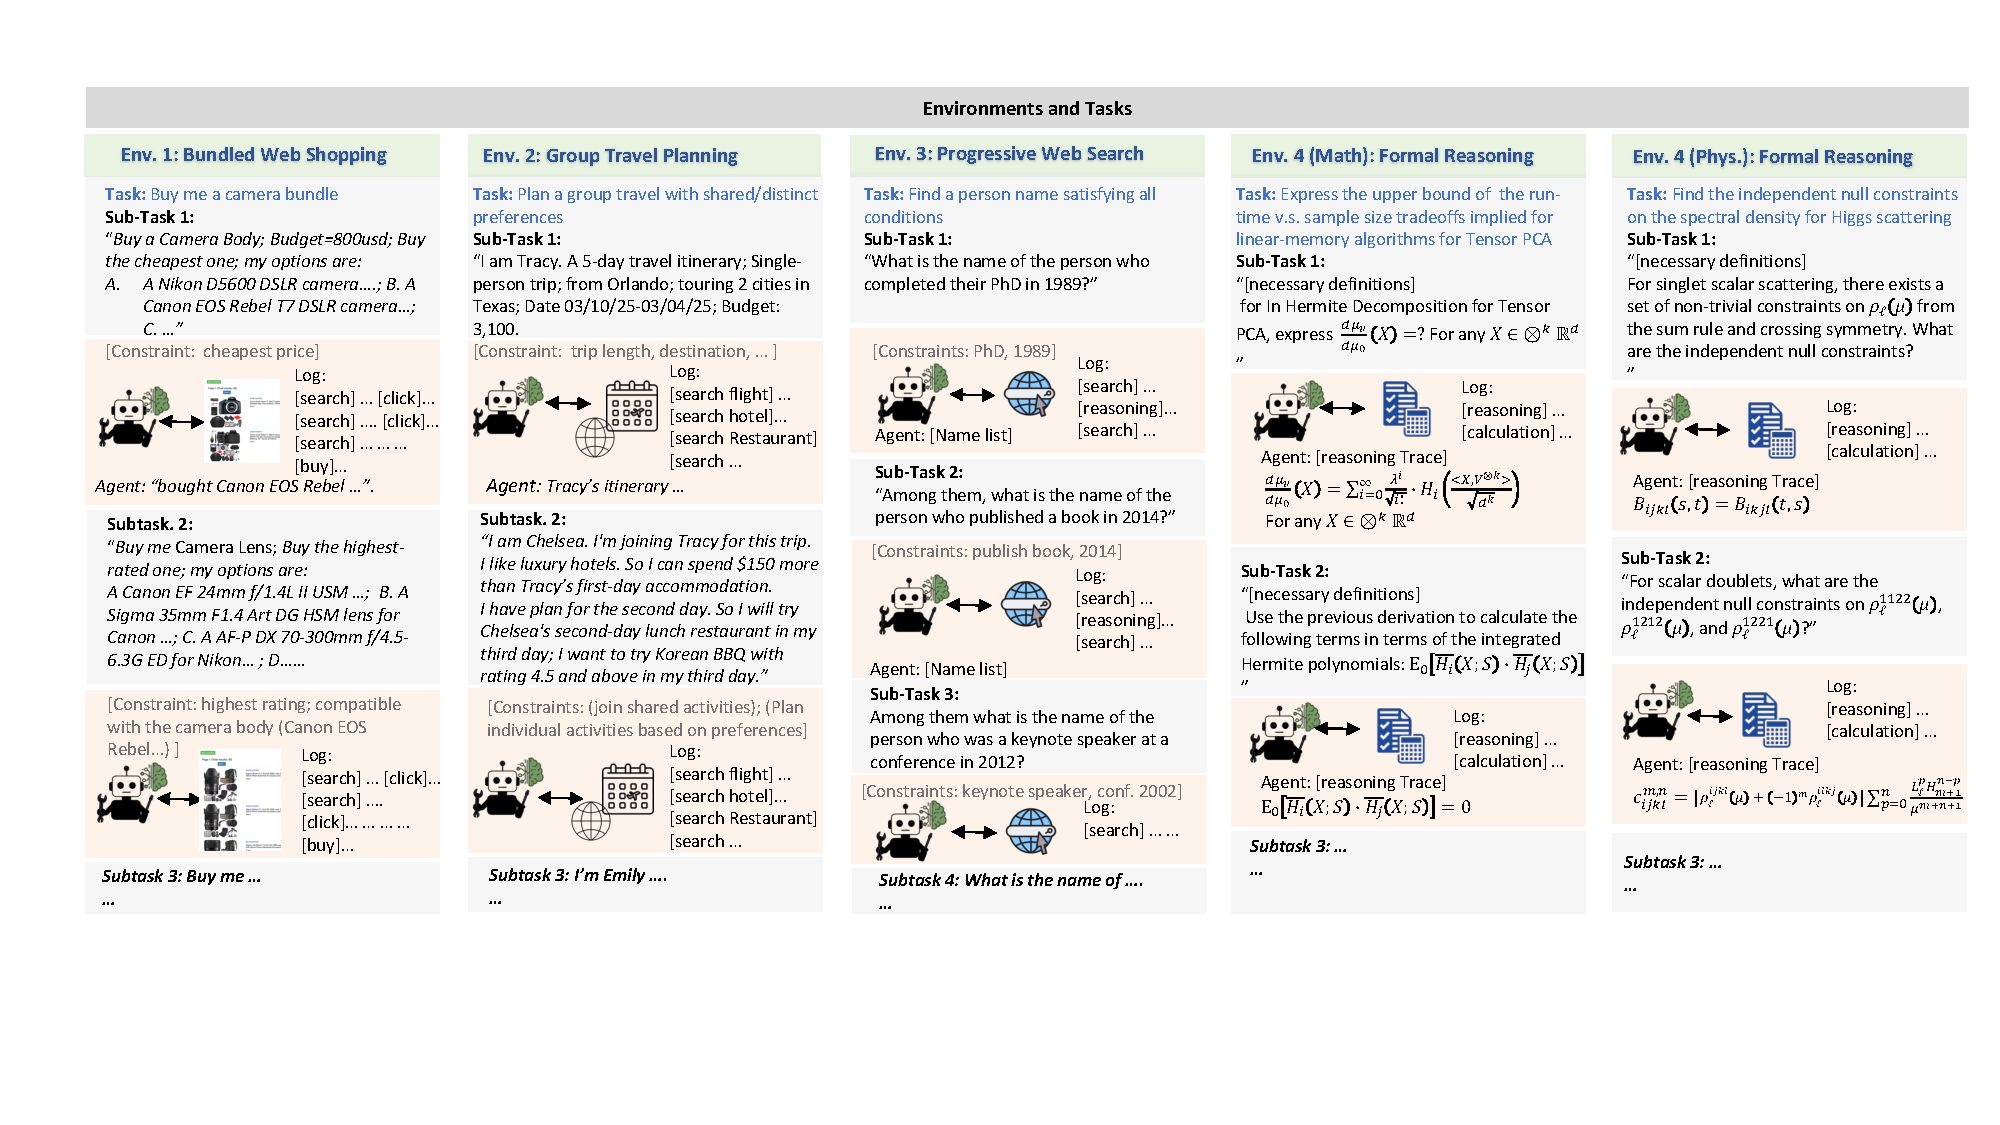
\includegraphics[width=\textwidth]{figs/main_memoryarena.pdf}
    \caption{\ours supports four distinct evaluation environments, where a memory-augmented task agent completes a sequence of interdependent subtasks. Each subtask session involves multiple agent actions.  }
    \label{fig:your_label}
    \vspace{-10pt}
\end{figure*}

\subsection{Task Composition and Data Preparation}
% Please add the following required packages to your document preamble:
% \usepackage{booktabs}
% \usepackage{graphicx}
\begin{table}[]
\resizebox{\linewidth}{!}{%
\begin{tabular}{@{}ccccc@{}}
\toprule
 &
  \textbf{\begin{tabular}[c]{@{}c@{}}\#min ST\\ (or Sess.)\end{tabular}} &
  \textbf{\begin{tabular}[c]{@{}c@{}}\#max ST\\ (or Sess.)\end{tabular}} &
  \textbf{\begin{tabular}[c]{@{}c@{}}\# avg T. \\ Trace L\end{tabular}} &
  \textbf{\begin{tabular}[c]{@{}c@{}}\# T (Groups \\ of Subtasks)\end{tabular}} \\ \midrule
\textbf{\begin{tabular}[c]{@{}l@{}}Bundled  Web Shopping\end{tabular}}    & 6          & \multicolumn{1}{c}{6}          & 41.5k          & 150         \\
\multicolumn{1}{r}{\textit{Included domain}}                                & \multicolumn{4}{r}{{[}\textit{Grocery,  Beauty, Electronics, Home Decor, Baking}{]}} \\
\begin{tabular}[c]{@{}l@{}}\textbf{Group } \textbf{Travel Planning}\end{tabular}            & 5          & 9                               & 40.6k          & 270         \\
\textbf{\begin{tabular}[]{@{}l@{}}Progressive Web Search\end{tabular}}  & 2          & \multicolumn{1}{c}{16}         & 122.4k         & 256         \\
\textbf{\begin{tabular}[c]{@{}l@{}}Math Formal Reasoning  \end{tabular}} & 2          & \multicolumn{1}{c}{16}         & 18.1k          & 40          \\
\multicolumn{1}{r}{\textit{Included Domains}            }                   & \multicolumn{4}{c}{\textit{[Pure math, Optimization, Learning theory]}} \\
\textbf{\begin{tabular}[c]{@{}c@{}}Phys. Formal Reasoning \end{tabular}} & 2          & 12                              & 14.1k          & 20          \\
\multicolumn{1}{r}{\textit{Included Domains}} &
  \multicolumn{4}{r}{\begin{tabular}[c]{@{}r@{}}{[}\textit{High energy theory,  High energy phenomenology},  \\ \textit{High energy lattice,  Condensed matter theory}{]}\end{tabular}} \\ \bottomrule
\end{tabular}%
}
% \vspace{0.2em}
\caption{Benchmark Statistics in \ours.}
\label{tab:stat}
\vspace{-15pt}
\end{table}
%Here, we introduce how we compose the tasks with multi-session subtasks. 
% \zexue{Need data statistics table}
\paragraph{Web Navigation: Bundled Web Shopping.} 
The Bundled Web Shopping environment models real-world shopping scenarios in which users purchase related products over time rather than in a single transaction. Later purchases depend on recalling attributes of earlier items to ensure compatibility and preference consistency.
We construct the Bundled Web Shopping environment by extending the shopping environment of \citep{yao2022webshop}, which contains tens of thousands of products with detailed descriptions and hierarchical category annotations. To reduce long-tail noise, we restrict our data to products from the five largest domains: Electronics, Home Decor, Baking, Beauty and Personal Care, and Grocery. Leveraging the category hierarchy, we first identify candidate groups of potentially compatible products by clustering items that share the same category path up to the penultimate level (for example, televisions from \textit{``Electronics $>$ Television \& Video $>$ Televisions $>$ TV Mounts, Stands \& Turntables''} and TV mounts from \textit{``Electronics $>$ Television \& Video $>$Televisions $>$ LED \& LCD TVs''} fall under the same category tree). This procedure yields coarse compatibility trees, serving as the structural basis to design bundle shopping instructions.

We then apply a fine-grained filtering process based on product features. We extract key attributes from product descriptions and construct \textit{accept–reject} maps that encode feature-level compatibility between product pairs using commonsense reasoning (e.g., a \textit{75-inch TV} accepts \textit{a stand with 70 inches long} but rejects \textit{a 50-inch stand}). These maps are used to form chains of compatible products across sessions and to generate auxiliary incompatible items as negative distractors. Human annotators then manually verify all compatibility chains and remove invalid combinations. Finally, annotators compose multi-session shopping instructions in which each session presents a mixture of incompatible distractors, compatible candidates, and an additional selection constraint (e.g., highest rating or highest price) to guarantee a unique compatible item is satisfied. Solving each session requires the agent to recall prior purchases, identify compatibility constraints, discard negative options, and select a valid product. Using this process, we construct 150 representative multi-session bundled shopping tasks as the final test set. More details in data creation are in Appendix.~\ref{appendix:data_shopping}.









%%%%%%%%%%%%%%%%%%%



\paragraph{Compositional Information Seeking: Progressive Web Search}
% [joanna's version] Starting with 830 entries from the BrowseComp-Plus dataset, we applied a two-stage filtering process to establish the final dataset. First, we focused on identifying challenging samples by first decomposing each query into multiple constituent sub-queries using the Negative Mining Query Decomposition Prompt. We then prompted the LLM to generate individual answers for every sub-query; these sub-queries and their corresponding generated answers were subsequently consolidated with the original query statement into a single prompt. By evaluating the LLM's response to this combined context, we performed an initial filter to retain only the "hard" instances that the model failed to answer correctly despite the provided sub-task breakdown.\\
% Second, we implemented a sequential prompting strategy on these remaining queries. For a query with $n$ sub-queries, we iteratively prompted the LLM from sub-query $1$ to $n-1$, where each step $i$ included the context of all previous sub-queries and their generated answers. Throughout this process, tool calls were restricted to documents specifically associated with the query. The final step combined the original query with the full sequence of sub-queries and answers to generate a terminal response. Only the instances resolved correctly through this sequential method were kept, resulting in a final dataset of 256 high-quality question-answer pairs.


We evaluate an agent’s ability to accumulate and reuse information across multiple search steps, where each step introduces an additional searching condition, and the final answer must satisfy all previously introduced conditions. Conceptually, this setting follows a form of \textit{progressive information seeking}, in which a user begins with a coarse specification of the target and incrementally adds new constraints over time, requiring the agent to retain and integrate information acquired in earlier searches.

Our test data builds upon BrowseComp-Plus~\citep{chen2025browsecomp}. Starting from its 830 entries, we apply a two-stage filtering and annotation process.
First, we evaluate the original entries using a large language model agent with access to web search tools, and remove instances that the agent can answer correctly in a single interaction. These filtered instances are solvable without retaining or recalling any information beyond the current prompt and tool responses, i.e., they do not require storing, accumulating, or reusing information across interactions and therefore place no demand on long-term memory.
% First, we directly execute each original BrowseComp-Plus query and remove the ``easy'' instances that can be correctly answered. This step filters out tasks that can be solved via short-term reasoning or tool calls alone, without requiring long-term memory to capture inter-query dependencies.
For the remaining instances,we decompose each query into a group of subqueries, where each subquery introduces one additional constraint. Note that search conditions are listed in parallel in BrowseComp-Plus. 
Therefore, all decomposed query groups undergo the second verification by human annotators. Annotators first assess whether the decomposition is semantically coherent, has no repetition, or other mistakes, and identify the correct search result for each subquery conditioned only on information available from preceding subqueries. If any subquery is unanswerable under these constraints (for example, if it depends on information introduced only in later subqueries), the entire group is discarded.
This process enforces a strict causal ordering among subqueries.
Finally, we retain 256 high-quality compositional search tasks with dependent subqueries and annotated answers as the test set in this task.

\vspace{-5pt}
\paragraph{Preference-constrained Planning: Group Travel}
%\zexue{@Churan, write how you create the data as detailed as possible}
%[churan's version] We construct our benchmark by extending the TravelPlanner dataset (train subset), which contains 45 single-person travel planning instances with ground-truth itineraries. We transform each instance into a multi-turn group travel scenario where the original traveler serves as the base person with a fixed plan, and 5 to 8 additional travelers join sequentially, forming groups of 6 to 9 people.
%Each day of the trip consists of fixed slots including breakfast, lunch, dinner, and accommodation. By default, new members follow the base person's itinerary since they travel as a group. However, during data construction, each slot for each traveler has a probability P of being assigned a personalized constraint, which takes one of two forms. JOIN constraints specify that a traveler wants to share an activity with another member (e.g., "I want to have dinner with Rebecca in our second day"), which uniquely determines the outcome. RELATION constraints define preferences relative to another member's choice, involving comparisons across dimensions such as price (absolute or percentage differences), rating, cuisine (set relations like intersection or subset), room type (same or different), and house rules. Each traveler can reference any preceding member, forming dependency chains up to depth 4.
%We generate 5 subsets based on maximum chain depth: M0 through M3 each contain 45 instances with maximum depths 0–3 respectively, while M4 contains 90 instances with depth 4, yielding 270 total instances. We design constraints to progressively narrow the candidate set, guaranteeing exactly one valid solution in the database. Finally, we use GPT-4.1-mini to polish the raw constraints into natural language while preserving all numerical values and logical relationships.

Our environment models realistic group travel scenarios in which an initial itinerary is planned by one traveler and additional participants join incrementally. More realistically, while group members may share common activities due to overlapping interests, they may also request individualized or partial-group arrangements when preferences diverge. Supporting such scenarios requires an agent to recall precisely previous activities and traveler preferences, and to reason about how new constraints interact with existing plans.

We build this environment based on TravelPlanner~\citep{xie2024travelplanner}, where a trip is represented as a sequence of daily activity slots (e.g., 3 meals, accommodations, sightseeing). We start with 45 single-traveler instances with a fully specified ground-truth itinerary. Then we transform each instance into a group travel scenario by treating the original traveler as a base participant with a fixed itinerary, and sequentially adding 5 to 8 additional travelers.

New travelers, by default, follow the base itinerary as shared group travel, but may specify personalized constraints that modify individual activity slots. These constraints take one of two forms. \texttt{JOIN} constraints specify that a traveler wishes to share a particular activity with another previously joined member (e.g., ``\textit{I want to have dinner with Rebecca on the second day}''), requiring the planning agent to assign the same activity choice to the later traveler. \texttt{RELATION} constraints define preferences relative to another member’s choice, expressed through comparisons along attributes such as price, rating, cuisine, room type, or house rules (e.g., ``I want to stay at a hotel with at least a two-level higher rating than Rebecca’s'').

All constraints are carefully designed to progressively narrow the feasible candidate set and guarantee \textit{a unique valid solution} in the underlying database. In total, we construct 270 group travel planning instances, where each traveler may reference or join any previous plans, forming dependency chains of up to depth four.


% We design this environment inspired by real-world cases where a person wants to join someone's trip after hearing their itinerary. In the natural case, travelers joined in one trip can have common activities based on common preferences, and are also allowed to conduct individual solo or partial-group activities if their interests are not aligned for specific items. Accurately planning a group of travel itineraries requires models to recall the previous scheduled activities/preferences and compare with the current person and reasoning. 

%We start with the existing TravelPlanner, where each day in the trip consists of a list of activity slots, such as breakfast, lunch, and dinner restaurants, accommodation, visiting activities, etc, based on the preference (we call it constraints here) specified when asking for an agent to plan a trip.  We take 45 single-person travel planning instances with ground-truth itineraries provided in the training set of TravelPlanner, then we transform each instance into a group travel scenario where the original traveler serves as the base person with a fixed plan, and 5 to 8 additional friend travelers join sequentially, in total forming groups of 6 to 9 people. In our data, new members by default follow the base person's itinerary since they travel as a group, but can specify their own personalized constraint.  The personalized constraints takes one of two forms: (1) JOIN constraints specify that a traveler wants to share an activity with another member who joined previously (e.g., ``I want to have dinner with Rebecca in our second day''),  in which case the outcome choice for that slot is the same (i.e., the same dinner restaurant at the same time with Rebecca). (2) RELATION constraints define preferences relative to another member's choice, involving comparisons across dimensions such as price, rating, cuisine, room type, and house rules (e.g., ``I want to stay in the hotel that at least 2-level higher than Rebecca's in the rating.'' 

%We carefully design constraints to progressively narrow the candidate set, guaranteeing exactly one valid solution in the database. Finally, we created 270 total group travel instances, where each traveler can join or reference any preceding member, forming dependency chains up to depth 4. This task can effectively evaluate how memory supports the agent in long-chain recalling, reasoning, and tool calling by jointly solving JOINT and RELATION constraints. 


\vspace{-5pt}
\paragraph{Sequential Formal Reasoning: Math \& Physics}
%\zexue{@Lang, write your data collection as detailed as possible }

%We analyzed academic papers in learning theory and differential geometry, and selected 40 papers into our dataset. The papers being selected must have clear main theoretical results with long-context mathematical notions, proofs or derivations. For those with multiple major theoretical results, we only select those whose verifications rely on long chains of preceding results.\\ 
%Each data sample contains two CSV files corresponding to one major theoretical result from a paper, which always has the title \textbf{Theorem}. Both files begin with all notations and necessary preliminaries for this major result; this part has no content that needs to be justified. The titles of those items include \textbf{Notations}, \textbf{Remark}, \textbf{Definition}, and \textbf{Algorithm}.\\
%After that, the preceding results of the main theoretical result are recorded in File 1. The names and indices of preceding results are mostly adopted from the original papers, and they are either \textbf{Lemmas} or \textbf{Propositions}, while occasionally some critical results are also named as theorems. To ensure self-consistency, the preceding results are recorded in the order so that the justifications of earlier results never depend on later results: For instance, if a lemma appears on row $k$, then its justification does not need any result appearing on row $\ell$ where $\ell > k$. This property is ensured by carefully reading all justifications. All preceding results and final result are recorded in the form of a question, and the answer key is located in a separated column. Some results in the papers, such as existence results, are difficult to be framed as questions so they are categorized as non-justifiable facts, instead of preceding results in File 1.\\
%File 2 contains all non-justifiable facts in File 1, and in addition only the final result.


The Formal Mathematical Reasoning environment is designed to reflect the structure and difficulty of research-level reasoning in scientific papers. Unlike standard math benchmarks that emphasize short, self-contained problems (e.g., AIME), major theoretical claims in fields such as learning theory and differential geometry typically depend on long-context arguments involving multiple intermediate results, definitions, and lemmas. Verifying a single claim often requires pages of derivations and careful reuse of previously established conclusions, making this setting a natural testbed for evaluating long-term memory and multi-step formal reasoning.

To construct this environment, we assemble a data creation team of senior PhD-level experts in theoretical mathematics and physics to manually curate and annotate academic papers with long and structured derivations. Experts review the papers,  select those whose central claims rely on extended chains of prior results, and decompose each central claim into an ordered sequence of intermediate statements (primarily lemmas and propositions) following the original structure of the source paper. Similarly, papers are discarded if the derivation lacks strict causal consistency, meaning that any statement depends on information introduced later in the argument.  For each remaining paper, experts record all necessary background required to justify each statement, such as notations, definitions, remarks, and algorithms. Each intermediate and final statement is then framed as a question with an expert-verified ground-truth answer, and the complete reasoning trajectory is recorded. Statements that are not naturally verifiable (e.g., existence assumptions) are provided as fixed facts to support subsequent reasoning. 


The final test set consists of 40 multi-question problems in mathematics and 20 in physics, each corresponding to a full derivation chain extracted from real research papers. The expert-curated derivation chains ensure high quality and introduce challenges well beyond existing math benchmarks, making this environment a rigorous test of both long-context memory and formal reasoning.


% The physics problems are selected from a wide range of topics including condensed matter and high energy theory and phenomenology, featuring various tasks in solving linear systems, differential equations, inequalities, and combinatorics. 
% The question set consists of several intermediate questions that breaks down the final one,
% or example questions that illustrate the methodology for the final question.

\subsection{Evaluation: Memory-Agent-Environment Loop}

%\textbf{Agent-Environment Loops.} \ours is a gym with multi-session agentic tasks with interdependent subtasks. In multi-session subtask interactions, we consider an \textit{LLM agent} $\mathcal{A}$ interacting with an \textit{environment} $\mathcal{E}$ over agentic tasks where each task consists of multiple interdependent subtasks:
% \begin{equation}
%     \mathcal{S}=\{s_1, s_2, ..., s_n\}
% \end{equation}

\textbf{Single-Session Agent-Environment Interactions.} 
When an \textit{LLM agent} $\mathcal{A}$ interact with an \textit{environment} $\mathcal{E}$ over certain agentic task $s$ (e.g., buy a camera lens),  the agent $\mathcal{A}$ interacts with $\mathcal{E}$ over a sequence of steps indexed by $t=1, ..., T_i$. At each step $t$, the agent selects an action (e.g., search the camera lens name) from its action space conditioned on the current instruction and the interaction history within the session, and the environment responds with an observation (e.g., show search results):
\begin{equation}
    a_{i,t} \sim  \pi_{\mathcal{A}}(\cdot | s, o_{i, 1:t-1}, a_{i, 1:t-1}), \quad o_{i_t} \in \mathcal{O}
\end{equation}
% So usually, the history interactions (trace) are provided as context in each step of the single-session task until task being terminated (e.g., bought one camera lens). 

In single-session tasks, the agent usually is provided with the complete interaction history (trace) as context at every step, until the task is terminated (e.g., after purchasing a camera lens).


%Using bundled web shopping as an example (e.g., buy a camera body with lens and cases), each subtask $s_i$ is executed as a separate \textit{session} (e.g., buy a camera lens). Within subtask $s_i$, the agent $\mathcal{A}$ interacts with $\mathcal{E}$ over a sequence of steps indexed by $t=1, ..., T_i$. At each step $t$, the agent selects an action (e.g., search the camera lens name) from its action space conditioned on the current subtask instruction and the interaction history within the session, and the environment responds with an observation (e.g., show search results):
% \begin{equation}
%     a_{i,t} \sim  \pi_{\mathcal{A}}(\cdot | s_i, o_{i, 1:t-1}, a_{i, 1:t-1}), \quad o_{i_t} \in \mathcal{O}
% \end{equation}
% So usually, the history interactions (trace) are provided as context in each step of an individual session (subtask) until the task is terminated (e.g., bought one camera lens). 

\textbf{Multi-session Agent-Environment Interactions.}
In real cases, a task may have multiple subtasks $S = \{s_i\}_{i=1}^n$, and subtasks are executed sequentially:
$[s_1 \rightarrow s_2 \rightarrow \cdots \rightarrow s_n]$.
Using bundled web shopping as an example (e.g., buy a camera body with lens and cases), each subtask $s_i$ is executed as a separate \textit{session}\footnote{Unless otherwise specified, we use the word \textit{session} and \textit{subtask} interchangeably} (e.g., first buy a camera body).
 While each session is temporally isolated, later subtasks may depend on information acquired in earlier ones (e.g., the version of the camera body bought before must be known when buying lens), motivating the need for a persistent state across sessions.

 \textbf{Final: Memory-Agent-Environment Loop.} 
We equip the agent $\mathcal{A}$ with a persistent memory system $\mathcal{M}$, which stores information across subtask sessions and is initialized as empty at the beginning of each evaluation episode. $\mathcal{M}$ can be a long-context buffer, a RAG system, or another memory agent. Usually, a memory system defines the two abstract functions\footnote{If the memory system is a long-context buffer, the retrieval function returns a concatenation of all past history, and the update function just appends the interactions of the current session into the buffer.}: (1) \textit{retrieval} which returns task-relevant memory given a query, and (2) \textit{update} which incorporates information from a completed subtask into $\mathcal{M}$. 

At each action step $t$ in subtask $s_i$, the agent retrieves relevant memory based on the current subtask, and actions are selected according to a memory-conditioned policy:
\begin{align}
    m_{i,t}&=\textsc{Retrieve}(\mathcal{M}, s_i, a_{i,1:t-1}, o_{i,1:t-1}). \\ a_{i,t} &\sim  \pi_{\mathcal{A}}(\cdot | s_i, o_{i, 1:t-1}, a_{i, 1:t-1}, m_{i,t})
\end{align}
Upon subtask completion, the memory system is updated as:
\begin{align}
    \mathcal{M} \leftarrow \textsc{Update}(\mathcal{M}, (o_{i,1:T}, a_{i,1:T}))
\end{align}
The updated memory is carried forward to the next subtask $s_{i+1}$, enabling information acquired in earlier sessions to influence future decision-making. We call it the \textit{Memory-Agent-Environment} Loop. 

In single-session execution, the agent–environment interaction implicitly follows a Memory-Agent-Environment loop, as the history of interactions added in the context of each action step can be viewed as the working memory of a single session. In such settings, persistent memory is not strictly required. In contrast, in multi-session settings,  subtasks are executed in separate sessions whose interaction traces are no longer directly accessible once a session terminates.  Task-relevant information must be selectively stored and retrieved through a persistent memory system in order to support decision-making in later subtasks. This explicitly enforces the Memory-Agent-Environment loop when the cumulative interaction trace spans multiple sessions and exceeds the scope of single-session context. 


%This Agent-Memory-Environment loop is necessary in multi-session settings where the entire trajectory across sessions is long and sparse, therefore requires a memory organization procedure. However, we would like to note that this loop is true in single-session as the history of interactions added to the context in each action step usually can be viewed as the working memory of a single session (i.e., the \textsc{update} is appending to the context window, the \textsc{retrieve} function is to return traces so far). Therefore, as a general setting to conduct long-horizon agentic tasks, Memory-Agent-Environment loop is the core evaluation princeple in \ours. 

 % The agent’s action selection is conditioned on the current subtask instruction and the interaction history within the session.
 
 
 % Our subtasks are constructed in a way that later sessions depend on information acquired in earlier ones, but do not explicitly restate this information.

% The Agent can also be coupled with \textit{a memory system} $\mathcal{M}$ ($\mathcal{M}$ can be a long-context buffer, a RAG system, or another memory agent), which is initialized as empty at the start of each evaluation task and persists across sessions. 

